%!TEX root = ../report.tex

% 
% Related work
% 
% (~17pgs)
\section{Related Work}

% começar por dizer como é que está organizada esta secção do trabalho e resumir de uma forma muito geral o que se fala em cada subsecção

This section presents the related work for this project and characterizes the main contributions of past works and how these contributions helped in the development of this project. This section is organized is three main parts: mHealth, mobile security and TrustZone.

The first part focuses on describing the attack surfaces of mHealth apps, the most common threats and their seriousness, present a few publicly available unsecure mHealth apps as well as some compliance recommendations that app developers should follow to avoid unnecessary security risks when handling sensitive health information. The second part of this sections describes the state-of-the-art of mobile security with a particular focus on the Android Operating System and how developers can build secure applications with a trusting \ac{OS} and security mechanisms built upon the application layer. The third part of the related work describes TrustZone, a hardware technology available in most modern \ac{ARM} processors which supports execution of two isolated worlds, a hardware-protected secure world and a normal world. Besides describing the technology, this sections also presents previous work developed using TrustZone and how these previous contributions may be helpful in achieving the main goals of this project. 

\subsection{mHealth}

As discussed above, mobile devices are increasing in number at astonishing rates and with this growth the mobile market becomes cheap and accessible. This motivates the shift from mainframe systems, located in the facilities of healthcare providers, to apps on mobile devices as well as storage in shared cloud services. This accessibility also motivates the private sector in building more healthcare applications to support both patients and healthcare agents. Thus, the mobile health market is becoming a competitive market and one which is increasingly handling more sensitive data.

%falar sobre as duas citations abaixo (ler os papers)

% THREAT TAXONOMY
Kotz, David \cite{kotz2011threat} defines a threat taxonomy for mHealth. In this paper the author categorizes threats into three main categories: \emph{Identity Threats}, \emph{Access Threats} and \emph{Disclosure Threats}.

Identity threats are described as mis-use of patient identities and include cases where a patient may lose (or share) their identity credentials, allowing malicious agents to access their \ac{PHR}. \emph{Insiders} (authorized \ac{PHR} users, staff of the \ac{PHR} organization, or staff of other mHealth support systems) may also use patient identities for medical fraud or for medical identity theft and \emph{outsiders} may be able to observe patient identity or location from communications.

Access threats are described as unauthorized access to \ac{PHR} and include cases where the patient, which controls the data, may allow broader-than-intended access or disclosure of information, \emph{insiders} who may snoop or modify patient data, with intents other than improving the healthcare of the patient, and even \emph{outsiders} which, by breaking into patient records, may leak or modify this data.

Disclosure threats include cases where an adversary captures network packets in order to obtain sensitive health data, this problem can be mitigated by using strong encryption methods, but even if the network traffic is encrypted it is possible to analyse the traffic to determine its characteristics \cite{wright2006inferring}. The adversary may also use physical-layer or link-layer fingerprinting methods to identify the device type and, because the wireless medium is open, an active adversary may inject frames or may selectively interfere with (cause collisions with) wireless frames. These methods may enable the adversary to create a man-in-the-middle situation, to use link-layer fingerprinting methods, or to compromise the devices in a way that divulges their secrets.

This work by Kotz, David \cite{kotz2011threat} helped in understanding what threats are inherent to mHealth systems and their development. An explicit set of rules for developing privacy-sensitive health applications was still needed to ease the development process. Avancha, Baxi and Kotz \cite{avancha2012privacy} filled the gap by surveying the literature, developing a privacy framework for mHealth and discussing the technologies that could support privacy-sensitive mHealth systems.

% PRIVACY FRAMEWORK FOR MHEALTH

This survey considers essential accounting for privacy in the design and implementation of any mHealth system, given the sensitivity of the data collected. A developer may use the list of privacy properties provided by this article as a check-list that should be considered in any design. Furthermore, a set of questions is left open for researchers to improve the efficiency and effect of these properties. It is also mentioned that the privacy challenges identified by this article need to be addressed with urgency, because mHealth devices and systems are being deployed now, and retrofitting privacy protections is far more difficult than building them in from the start.

% SECURITY CONCERNS MHEALTH ANDROID
% ler os papers citados aqui
He, Dongjing, et al. \cite{he2014security} analyse several mHealth applications available in Android's app store contributing to the understanding of security and privacy risk on the Android platform.

In this paper, three studies were made with the following goals:
\begin{itemize}
	\item \textbf{Study 1: What are the potential attack surfaces?}
	\item \textbf{Study 2: How widespread is the threat?}
	\item \textbf{Study 3: How serious is the threat?}
\end{itemize}

% ler os papers citados aqui
 In the first study 160 apps are analysed to find evidence of threats. From analysing previous literature \cite{zhou2013identity,naveed2014inside,aviv2012practicality,cai2012practicality,chin2011analyzing,fsecure,sevenwaystohangyourselfwithandroid}, seven attack surfaces are determined to be in need of protection. These seven attack surfaces are shown in table \ref{tab:attacksurfaces}.

\begin{table}[t]
	\caption {Description of attack surface (taken from He et al. \cite{he2014security})}
	\label{tab:attacksurfaces}
	\begin{tabular}{|>{\raggedright}p{2cm}|>{\raggedright\arraybackslash}p{10cm}|}
		\hline
		\textbf{Attack Surface}      & \textbf{Description}                                                                                                                    \\ \hline
		Internet            & Sensitive information is sent over the internet with unsecure protocols (e.g. HTTP), misconfigured HTTPS, etc.                 \\ \hline
		Third Party         & Sensitive information is stored in third party servers                                                                         \\ \hline
		Bluetooth           & Sensitive information collected by Bluetooth-enabled health devices can be sniffed or injected                                 \\ \hline
		Logging             & Sensitive information is put into system logs where it is not secured                                                          \\ \hline
		SD Card Storage     & Sensitive information is stored as unencrypted files on SD card, publicly accessible by any other app                          \\ \hline
		Exported Components &  Android app components, intended to be private, are set as exported, making them accessible by other apps                     \\ \hline
		Side Channel        & Sensitive information can be inferred by a malicious app with side channels, e.g. network package size, sequence, timing, etc. \\ \hline
	\end{tabular}
\end{table}
%\FloatBarrier

% AQUI ESTOU A DIZER TBM QUE ESCOLHI A APPLICACAO A FAZER POR CAUSA DESTES NUMEROS
In this study the authors also document that the 160 apps studied target two different audiences: 129 (81.65\%) are for patients, 32 (20.25\%) are for healthcare professionals and the remaining 3 (1.90\%) are targeted for both. Most apps targated for patients (60\%) are in the Life Management category followed by apps that manage and synchronize user health information (\ac{PHR} Management) which occupy nearly half (46.88\%) of these apps. These numbers are a good indicator of what data is handled by most commercial mHealth apps available and motivate the choice made to build a \ac{PHR} Management app as demo for TrubiZone.

A few examples of vulnerable applications are also revealed during this study. Regarding unencrypted information sent over the Internet, Doctor Online \cite{doctoronline} (patients can talk to doctors online) and Recipes by Ingredients \cite{recipesbyingredients} send unencrypted sensitive information, including the user's email and password, in clear text. With regard to logging sensitive information, the study pinpoints CVS/pharmacy \cite{cvspharmacy}, which logs the prescription refill details from user inputs, including name, email address, store number, and Rx number and also logs user login credentials in a debug log message. A malicious party can use this information to view user profiles, prescription history, which could support medical identity theft, and it is even possible to do online pharmacy shopping with user's stored credit card information. Further applications are given as example for exposing sensitive information, Noom Weight Loss Coach \cite{noomwlc} reveals user workout history by exposing its Content Providers to external apps, which means any app can access the exposed Content Providers without declaring any permission. Finally, this first study concludes with the example of sleep monitoring apps, such as SnoreClock \cite{snoreclock} and Sleep Talk Recorder \cite{sleeptalk}, which store the sleep records of users as unencrypted audio files on external storage. With read permission for the SD card, as well as internet permission, a malicious app can read a user's sleep recordings and even send them to remote servers.

In the second study, 27 apps of the top 1080 free apps from the Medical and Health \& Fitness categories on Google Play were analysed according to their vulnerabilities. From this analysis, three attack surfaces are identified as the most important ones: \emph{Internet}, \emph{Third Party Services} and \emph{Logging}. Only 7 of these 27 apps use the Internet to effectively send medical information over to remote servers. It is important to understand if the information sent over the Internet is protected. To achieve this, the authors captured network traffic and concluded that only 57.1\% (4/7) of these apps use encrypted communication and the remaining 42.9\% (3/7) use unencrypted communication to send sensitive health information. Among the unencrypted contents sent by these 3 apps were emails, usernames and passwords. This study also concludes that 85.7\% (6/7) of these apps are hosted and store the recorded data on third party servers. This is an economical and scalable solution for mobile applications, but storing sensitive health records on third party servers can have serious implications, mostly due to app users not being aware that their data is being stored on third party servers and because these users are not able to tell if this data is stored encrypted in such a way that hosting companies do not have access to it.

Some health apps use Bluetooth devices to collect personal health information such as heart rate, respiration, pulse oximetry, electrocardiogram (ECG), blood pressure, body weight, body temperature, quality of sleep and exercise activities. Naveed et al. \cite{naveed2014inside} show how a malicious app can stealthily collect user data from an Android device or spoof a device and inject fake data into the original device's app, in what is called an \ac{DMB} attack. One of the 27 apps analysed in this study connects to external health sensors and uses default PIN code 0000, which makes it vulnerable to the \ac{DMB} attack. Along with the logging, external storage, exported components and the other problems discussed above, which represent the explicit channels used for attacks, side channels can be exploited by a malicious party to infer sensitive information from apps, even when they are well-designed and implemented. This study mentions an example by Zhou et al. \cite{zhou2013identity} where a correlation between network payload size and the disease condition a user selects on WebMD mobile \cite{webmd}. Network payload size is publicly accessible in Android, which represents a problem when such correlations can be made. Zhou et al. \cite{zhou2013identity} mitigate the problem by modifying the Android kernel to enforce limitations on accessing Android public resources. 

In the third study, another 22 apps, which send information over the Internet, are randomly selected from the same top 1080 apps and used to understand the seriousness of the threat. The 22 apps are analysed to understand what information is effectively being sent over the Internet and the conclusion is that when used as intended these apps gather, store and transmit a variety of sensitive user data which includes at least personal profiles, health sensor data, lifestyle data, medical information browsing history and third-party app data (e.g. Facebook account information). Figure \ref{fig:sensitivedistribution} shows the distribution of sensitive data in the 22 apps. Consequences of data breaches, information disclosure or tempering with sensitive health data depend on the type, sensitivity and volume of the data breached, but it is clear that profiling, medical identity theft and healthcare decision-making errors are all possible. This is why the authors suggest the use of encryption for communication and storage, and encourage developers to create a set of security and privacy guidelines that offer a baseline for protection.

\begin{figure}[t!]
  \centering
  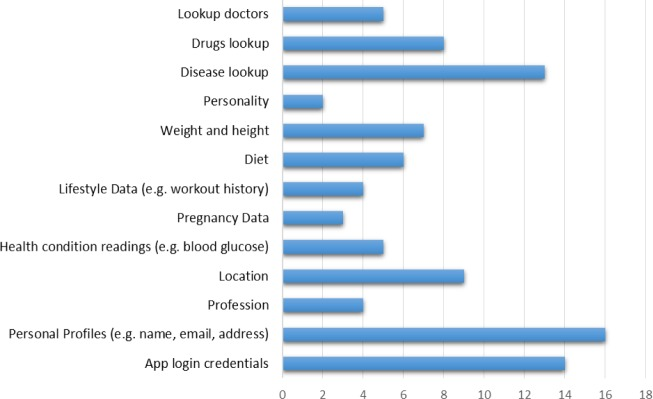
\includegraphics[width=0.95\textwidth]{img/sensitivedistribution.jpg}
  \caption{Sensitive information distribution for study 3 (taken from  He et al. \cite{he2014security})}
  \label{fig:sensitivedistribution}
\end{figure}
%\FloatBarrier

% EM QUE O TRABALHO ME AJUDOU
The work by He, Dongjing, et al. \cite{he2014security} helped in understanding what are the most common attack surfaces when considering mHealth applications on Android and it also helped assessing the security risks inherent to applications handling privacy sensitive information. This paper generally describes the state-of-the-art of security in commercial mobile health apps and pinpoints what should be fixed in order to build better and more secure application for the healthcare industry. It is clear that developers focus much more on building feature-full applications rather than secure apps and this is why it is important to build a framework which allows developers to completely focus on the features they want to provide without having to focus heavily on security. We believe that building a developer framework over ARM's TrustZone technology is a good solution because with TrustZone is possible to fully enjoy the potential of the hardware already available in most mobile devices. This technology will be described in section \ref{sec:trustzone}. 

\subsection{Mobile Security Mechanisms}

This section describes the security mechanisms available for the Android platform, either from native Android or as security extensions, and how these mechanisms can be used to solve some of the problems covered in the previous section. Work by Duarte, Nuno \cite{nunoduarte} and Costa, Miguel \cite{miguelcosta} extensively describe Android's security mechanisms and divide them in seven groups: \emph{(i)} digital rights management, \emph{(ii)} access control mechanisms, \emph{(iii)} permission refinement, \emph{(iv)} application API security, \emph{(v)} privacy enhancement systems, \emph{(vi)} access control hook APIs, and \emph{(vii)} memory instrumentation. We suggests the addition of a new security mechanism: \emph{(viii)} TrustZone technology. This last mechanism is not directly related to Android but, with a significant presence in most modern smartphones, its discussion is imperative for this project. Enck et al in is work "Understanding Android security" \cite{enck2009understanding}.%as well as \textbf{MORE REFERENCES HERE}, which are good sources for information on this section of related work.

\subsubsection{Digital Rights Management}
The first security mechanism analysed is Digital Rights Management. This specific access control technology allows data owners to restrict if and how their data is copied and also how that data is handled once transferred to another device. The \ac{DRM} ecosystem is composed of the following entities:

% estruturar melhor esta lista
\begin{itemize}
	\item \emph{User} - human user of the DRM Content
	\item \emph{Content Issuer} - entity that delivers the content
	\item \emph{Rights Issuer} - entity responsible for assigning permissions and constraints to \ac{DRM} content
	\item \emph{Rights Object} - XML document generated by a Rights Issuer expressing the restrictions associated to the content.
	\item \emph{\ac{DRM} Agent} - trusted entity responsible for enforcing permissions and constraints upon the \ac{DRM} content
\end{itemize}

\ac{DRM} can be used to protect proprietary software, hardware or general content. The most common application for \ac{DRM} nowadays is music and video games, because these represent highly valuable intellectual property. To understand how \ac{DRM} works in the context of mHealth one can suggest a simple example of a \ac{PHR} mobile health application. In this scenario, the healthcare provider (e.g. a hospital) would be the \emph{content issuer}, and it would use a \emph{rights issuer} to assign the restrictions imposed upon the \ac{DRM} content, which in this case would be the personal health records of a patient, when this content is transferred to the patient's device. When using \ac{DRM}, the patient is limited to access the content through a \emph{\ac{DRM} Agent}.

The \ac{OMA} developed a DRM standard \cite{drm} which defines the format of the content delivered to DRM Agents, as well as the way this content can be transferred from the Content Issuer to the DRM Agent. For DRM to be effective this standard must be complied by mobile operators, device manufacturers and middleware developers. Android provides an extensible DRM framework, called Android DRM Framework \cite{androidDRM}, allowing application developers to enable their apps to manage rights-protected content by complying with one of the supported DRM schemes (specific mechanisms, enforce by DRM Agents, to handle particular types of files).

This mechanism can be useful for protecting personal healthcare records by restricting the way data can be copied and handled. For this project however, DRM is not enough to ensure the confidentiality, integrity and availability of the sensitive data because it may fail to do so when the operating system is compromised with a malicious agent.

\subsubsection{Access Control Mechanisms}

Access control mechanisms is a security model in which subjects (e.g. user, processes, threads, etc.) can perform actions on the system, namely on resources (e.g. files, sensors, etc.), typically called objects. Android follows a type of access control references as \ac{DAC}, heritage from it's Linux based kernel. In a \ac{DAC} system the data owner is responsible for the data and thus determines who can access the data he owns. In a Linux systems, one can image a system administrator creating several files and allowing access to these files according to certain permissions. In this example, a subject with the specified permissions may access the file like its owner intended. In Android we can think of a similar example, since an application can create and store files in the filesystem, thus becoming the sole owner of these files, it can allow access to these files to any other application it wishes.

Although Android inherits the \ac{DAC} from its Linux ancestry, most other resources in Android follow \ac{MAC} policies. In \ac{MAC}, subjects are much more restricted in determining who has access to their resources. An example of this from the physical security field are the levels: confidential, secret and top secret. These labels are the only resource available to define the level of clearance of subjects or to classify data. If a subject attempts to access a classified piece of data a verification is done to assess if this subject's security level matches (or is above) that of the classified piece of data. Similarly in Android, once a subject attempts to access an object, it triggers a policy evaluation by the kernel, which assesses whether the access may be granted. The advantage of this strict system is its robustness, because subjects cannot override or modify the security policy. In Android, applications must specify in their manifests the permissions they require at runtime and after the installation neither applications nor users have any control over the access policies.

%Reescrever esta frase por mim
Because \ac{MAC} is robust, several systems were created over the years to extend Android's access control model. SEAndroid \cite{smalley2013security} solves problems related to resources complying with the \ac{DAC} mechanism. The authors ported SELinux \cite{peter2001integrating} to provide \ac{MAC} at the kernel layer. The kernel was then modified to support a new \ac{MAC} policy (e.g., filesystem, IPC) and a new middleware layer (MMAC) created to extend \ac{MAC} to Android's Binder IPC. TrustDroid \cite{bugiel2011practical} extends the \ac{MAC} mechanism to all the platform's resources (e.g., filesystem which complied with DAC) inorder to isolate different domains' sensitive information.

Even though access control mechanisms allow isolation between different subjects in a system, thus enforcing the confidentiality and integrity needed for this project, it still relies on the premise that the underlying middleware and kernel are secure. With this assumption sensitive data may be at risk when the \ac{TCB} is compromised. For this reason access control mechanisms are not sufficient to ensure the security needs of this project.  

\subsubsection{Permission Refinement}

\subsubsection{Application API Security}

\subsubsection{Privacy Enhancement Systems}

\subsubsection{Access Control Hook APIs}

\subsubsection{Memory Instrumentation}

\subsubsection{ARM TrustZone Technology}

\subsubsection{Summary}

Aqui falar sobre a tabela \ref{tab:securityMechanismsComparison} e concluir finalmente que temos que olhar para o trustzone pois é destes mecanismos o que parece mais adequado.

% Please add the following required packages to your document preamble:
% \usepackage{graphicx}
\begin{table}[htbp!]
	\centering
	\caption{Comparison between security mechanisms with and without a compromised Operating System (Android).}
	\label{tab:securityMechanismsComparison}
	\resizebox{\textwidth}{!}{%
		\begin{tabular}{|l|l|l|l|l|}
			\hline
			Security Mechanism          & Confidentiality & Data Integrity & Availability & Malware \\ \hline
			Digital Rights Management   & \cmark          & \cmark         & \cmark       & \xmark  \\ \hline
			Access Control Mechanisms   &                 &                &              & \xmark  \\ \hline
			Permission Refinement       &                 &                &              & \xmark  \\ \hline
			Application API Security    &                 &                &              & \xmark  \\ \hline
			Privacy Enhancement Systems &                 &                &              & \xmark  \\ \hline
			Access Control Hooks        &                 &                &              & \xmark  \\ \hline
			Memory Instrumentation      &                 &                &              & \xmark  \\ \hline
			TrustZone Technology        & \cmark          & \cmark         & \cmark       & \cmark  \\ \hline
		\end{tabular}
	}
\end{table}

% TRUSTZONE
\subsection{TrustZone}
\label{sec:trustzone}





